\section{WS5: Autonomomous hover flight of two drones}
\label{section:ws5}

In order to hover more than a single drone a special launch file is needed. It is similar to having multiple launch file for a single drone in a single file. A new launch file named \textit{hover\_multiple.launch} is created 
\begin{mdframed}[backgroundcolor=light-gray, linecolor=light-gray]
\begin{verbatim}
$ cd ~/crazyflie_ws/src/crazyflie_ros/crazyflie_demo/launch
$ nano hover_multiple.launch
\end{verbatim}
\end{mdframed}

\noindent to which the following content is added:
\begin{code}
\begin{minted}[breaklines, linenos, frame=single]{xml}
<?xml version="1.0"?>
<launch>
  <arg name="joy_dev" default="/dev/input/js0" />

  <arg name="uri1" default="radio://0/100/2M/E7E7E7E701" />
  <arg name="frame1" default="crazyflie1" />
  <arg name="x1" default="3.5" />
  <arg name="y1" default="1.5" />
  <arg name="z1" default="0.4" />
  
  <arg name="cf_id1" default="111" />
  <arg name="stream_port1" default="11111" />

  <arg name="uri2" default="radio://0/100/2M/E7E7E7E702" />
  <arg name="frame2" default="crazyflie2" />
  <arg name="x2" default="2.5" />
  <arg name="y2" default="1.5" />
  <arg name="z2" default="0.4" />
  
  <arg name="cf_id2" default="222" />
  <arg name="stream_port2" default="22222" />

  <include file="$(find crazyflie_driver)/launch/crazyflie_server.launch">
  </include>

  <node name="joy" pkg="joy" type="joy_node" output="screen">
    <param name="dev" value="$(arg joy_dev)" />
  </node>

  <group ns="crazyflie1">
    <include file="$(find crazyflie_driver)/launch/crazyflie_add.launch">
      <arg name="uri" value="$(arg uri1)" />
      <arg name="tf_prefix" value="crazyflie1" />
      <arg name="enable_logging" value="False" />
    </include>

    <node name="joystick_controller" pkg="crazyflie_demo" type="controller.py" output="screen">
      <param name="use_crazyflie_controller" value="True" />
      <param name="joy_topic" value="/joy" />
    </node>

    <include file="$(find crazyflie_controller)/launch/crazyflie2.launch">
      <arg name="frame" value="$(arg frame1)" />
    </include>

    <node name="pose" pkg="crazyflie_demo" type="publish_pose.py" output="screen">
      <param name="name" value="goal" />
      <param name="rate" value="10" />
      <param name="x" value="$(arg x1)" />
      <param name="y" value="$(arg y1)" />
      <param name="z" value="$(arg z1)" />
    </node>
    
    <!-- run servicelayer_gps_ros -->
    <node name="gps_1" pkg="servicelayer_gps_ros" type="GPS" args="$(arg cf_id1) $(arg frame) $(arg stream_port1)" />
    
  </group>

  <group ns="crazyflie2">
    <include file="$(find crazyflie_driver)/launch/crazyflie_add.launch">
      <arg name="uri" value="$(arg uri2)" />
      <arg name="tf_prefix" value="crazyflie2" />
      <arg name="enable_logging" value="False" />
    </include>

    <node name="joystick_controller" pkg="crazyflie_demo" type="controller.py" output="screen">
      <param name="use_crazyflie_controller" value="True" />
      <param name="joy_topic" value="/joy" />
    </node>

    <include file="$(find crazyflie_controller)/launch/crazyflie2.launch">
      <arg name="frame" value="$(arg frame2)" />
    </include>

    <node name="pose" pkg="crazyflie_demo" type="publish_pose.py" output="screen">
      <param name="name" value="goal" />
      <param name="rate" value="10" />
      <param name="x" value="$(arg x2)" />
      <param name="y" value="$(arg y2)" />
      <param name="z" value="$(arg z2)" />
    </node>
    
    <!-- run servicelayer_gps_ros -->
    <node name="gps_2" pkg="servicelayer_gps_ros" type="GPS" args="$(arg cf_id2) $(arg frame) $(arg stream_port2)" />
  </group>
  
</launch>

\end{minted}
\caption{ROS launch file for hovering two drones\\}
\label{listing:xml_multi_hover}
\end{code}

\noindent This launch file defines all the nodes required to run for hovering two drones. The main difference from the crazyflie ros stack being that a modified Optitrack server is used for position estimate instead of Vicon or VRPN. The next step is to launch the newly created configuration and observe if the drones would hover.\\
\noindent The following command is issued:
\begin{verbatim}
$ roslaunch crazyflie_demo hover_multiple.launch
\end{verbatim}
The "O" button on the PS4 gamepad is pressed for the drones to take off and it can immediately be see that only the drone named "crazyflie2" takes flight and is hovering while the first drone (crazyflie1) remains static throughout the whole test. At the first test the source of this issue was related to ROS as launching two \texttt{servicelayer\_gps\_ros} nodes was leading to the first one to be closed with an error message reporting that another node is created with the same name.\\
\noindent Assigning different name to the node in the launch file above removes the error message but still only the second drone is able to operate. This is where it was revealed that connecting to the Optitrack gps sever using the same streaming port causes one of the connections to close. This lead to introducing the ability to choose a different streaming port as described in Listing \ref{listing:servicelayer_tf_frames} and using different ports as arguments for the \textit{hover\_multiple.launch} file.\\
However only one of the drones is able to hover, the other one seemingly does not receive any commands.\\
To investigate this, two drones are put in the SmartCity layout named "RigidBody 111" for "crazyflie1" and "RigidBody 222" for "crazyflie2". The following commands are executed:
\begin{verbatim}
$ rosrun servicelayer_gps_ros GPS 111 crazyflie1 11111
\end{verbatim}

\noindent and in a new terminal run:

\begin{verbatim}
$ rosrun servicelayer_gps_ros GPS 222 crazyflie1 22222
\end{verbatim}

\noindent The result that can be seen after issuing these commands is that the Optitrack GPS server does not allow connecting by other means than the standard ports. Further attempt to connect two clients from the same pc by using different streaming ports or even gps ports are unsuccessful as only one instance can remain running. The conclusion is that the Optitrack server is designed to accept connection from distinct systems rather than multiple connections from the same computer. Resolving this issue requires modifying the source code of the server but this approach is not desired since multiple parties not related to this project are using it.\\
The nest step is to attempt to modify the source code of the VRPN client discussed in Section \ref{section:ws3}.

\subsection{Using a modified VRPN client for position estimate}
As described in Section \ref{section:ws3}, the position estimate provided by the VRPN client doesn't allow the drones to be operated autonomously due the the the $x,y,z$ axes being switched.\\
\noindent It is not possible to modify the source code of the VRPN client that is installed according to instruction from \cite{HoenigMixedReality2015} (by using apt-get) as only the compiled binaries are provided. For this attempt the previously installed binaries are removed and the client is built from source by first checking out the official repository from \cite{web_vrpn_git}:
\begin{verbatim}
$ cd ~/crazyflie_ws/src
$ git clone https://github.com/ros-drivers/vrpn_client_ros.git
\end{verbatim}

\noindent Before building the package the following file is edited:
\begin{verbatim}
$ cd vrpn_client_ros
$ nano src/vrpn_client_ros.cpp
\end{verbatim}

\noindent In the \textit{handle\_pose()} several lines are modified as shown below:
\begin{minted}[breaklines, frame=single]{cpp}
void VRPN_CALLBACK VrpnTrackerRos::handle_pose(void *userData, const vrpn_TRACKERCB tracker_pose)
{
  //...
  tracker->pose_msg_.pose.position.x = tracker_pose.pos[2];
  tracker->pose_msg_.pose.position.y = tracker_pose.pos[0];
  tracker->pose_msg_.pose.position.z = tracker_pose.pos[1];
  
  tracker->pose_msg_.pose.orientation.x = 0;
  tracker->pose_msg_.pose.orientation.y = 0;
  tracker->pose_msg_.pose.orientation.z = tracker_pose.quat[1];
  tracker->pose_msg_.pose.orientation.w = tracker_pose.quat[3];
  
  //...
  
  tracker->transform_stamped_.transform.translation.x = tracker_pose.pos[2];
  tracker->transform_stamped_.transform.translation.y = tracker_pose.pos[0];
  tracker->transform_stamped_.transform.translation.z = tracker_pose.pos[1];
  
  tracker->transform_stamped_.transform.rotation.x = 0;
  tracker->transform_stamped_.transform.rotation.y = 0;
  tracker->transform_stamped_.transform.rotation.z = tracker_pose.quat[1];
  tracker->transform_stamped_.transform.rotation.w = tracker_pose.quat[3];
}
\end{minted}

\noindent The purpose of these edits is to swap the translation and rotation axes so that the tracked bodies are perceived correctly in the SmartCity layout. The choice of which axes to swap is done in accordance with Table \ref{table:smartcity-to-optitrack}. As mentioned before $roll$ and $pitch$ values are reported unreliably by Optitrack. In addition to this the crazyflie ros stack controller uses $x, y, z$ and $yaw$ to control the position of the drone. For these two reasons the quaternion values for the $x$ and $y$ axes have been set to zero.

\noindent The last thing to do before building is to create a launch file for the VRPN client:
\begin{verbatim}
$ cd ~/crazyflie_ws/src/vrpn_client_ros/launch
$ nano vrpn.launch
\end{verbatim}

\noindent with the following contents:
\begin{minted}[breaklines, linenos,frame=single]{xml}
<launch>

  <arg name="server" default="192.168.0.100"/>

  <node pkg="vrpn_client_ros" type="vrpn_client_node" name="vrpn_client_node" output="screen">
    <rosparam subst_value="true">
      server: $(arg server)
      port: 3883

      frame_id: world
      broadcast_tf: true

      # Must either specify refresh frequency > 0.0, or a list of trackers to create
      #refresh_tracker_frequency: 1.0
      #trackers:
      - crazyflie1
      - crazyflie2
    </rosparam>
  </node>
</launch>
\end{minted}

\noindent It is almost the same file as described in Section \ref{section:ws3} with the exception that not all objects available to Optitrack are tracked but just the drones that are of interest. Since VRPN doesn't require to keep a naming scheme the two testing drones are renamed to "crazyflie1" and "crazyflie2" in the Optitrack Motive interface.
At this point the launch file used in Listing \ref{listing:xml_multi_hover} can be modified to use the modified VRPN client. This can be done by removing or commenting line 54 and line 82 so it doesn't use the \textit{servicelayer gps} and instead add the following line, just before the closing \texttt{</launch>} at the end of the file:
\noindent with the following contents:
\begin{minted}[breaklines ,frame=single]{xml}
  <!-- run vrpn client -->
  <include file="$(find vrpn_client_ros)/launch/vrpn.launch"/>
\end{minted}

\noindent Once this done, ensure the launch file contains the correct drone starting positions and that the gamedpad and CrazyRadio PA are connected. The package is built and run as such:
\begin{verbatim}
$ cd ~/crazyflie_ws/
$ catkin_make
$ roslaunch crazyflie_demo hover_multiple.launch
\end{verbatim}

\noindent At this time pressing the "takeoff" gamepad button results in both drones taking off and hovering at their given points. The plotted path of the $z$-axis of both drones can be seen in Figure \ref{figure:hover_multiple}

\begin{figure}[H]
\centering
 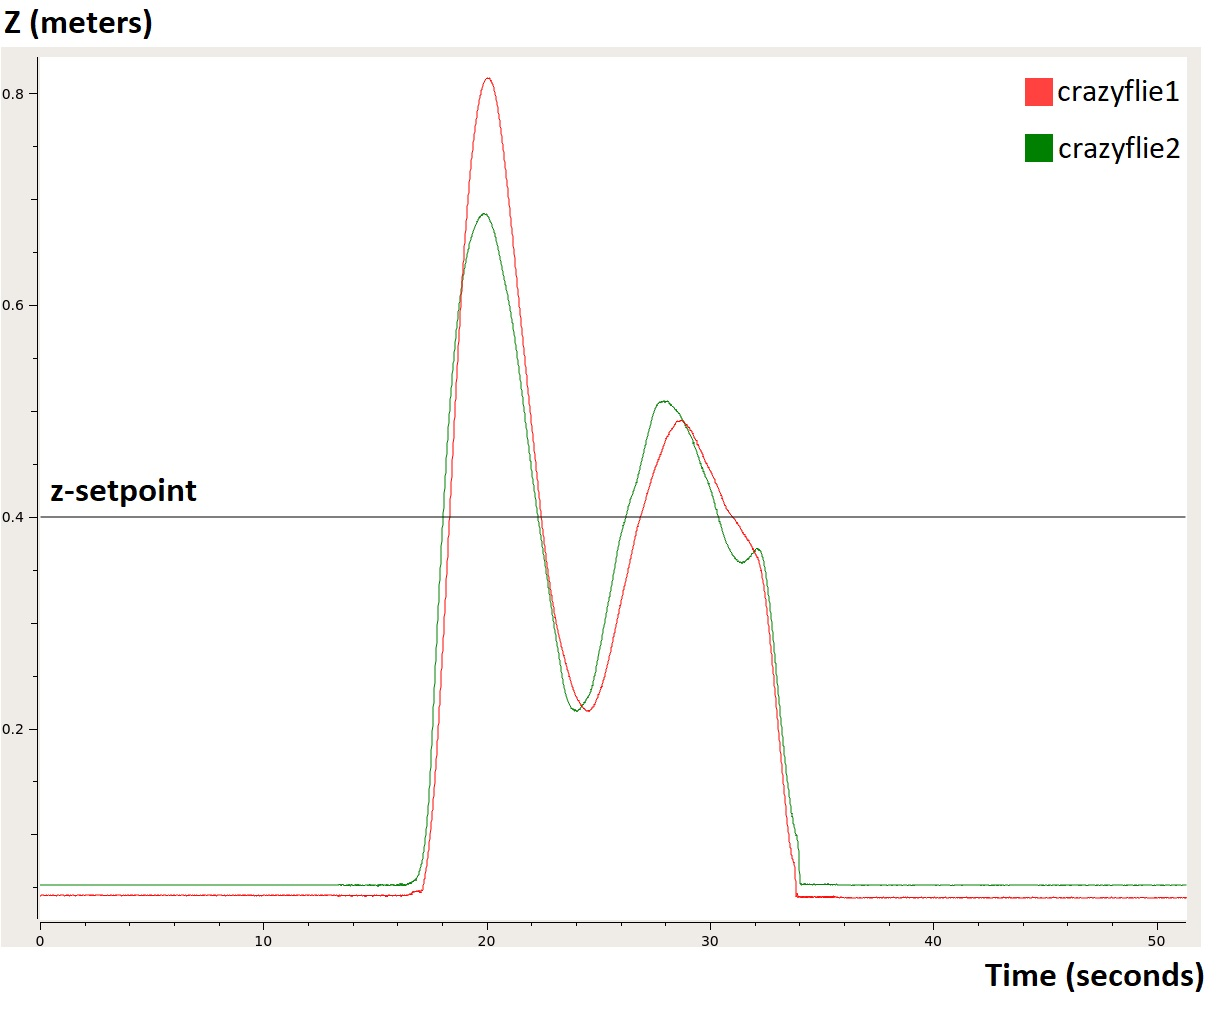
\includegraphics[scale=0.25]{Figures/hover_multiple.jpg}
 \caption{Plotted z position of two drone commanded to hover at the 0.4 meter point on the z-axis}
 \label{figure:plot_hover_multiple}
\end{figure}.

\noindent Similar to the single drone flight, the drones are issued the takeoff command at time zero and landing is requested after about 32 seconds. The test shows that the drones are able to hover around the setpoint with a deviation of up to 40 centimetres. The $x,y$ axes are not plotted as the tests are only aiming at controlling the position on the $z$ axis. The crazyflie ros stack position controller handles the $x,y,z$ and $yaw$ position of the drone which means that the drone hovers 0.4 metres above the point it took flight from if these coordinates are entered in the launch file as seen in Listing \ref{listing:xml_multi_hover}.



